% CREATED BY DAVID FRISK, 2018
% Title page and last page updated by Magnus Gustaver, 2020
% Updates in Settings and addition of Acronyms and Nomenclature templates by Kyriaki Antoniadou-Plytaria, 2021


% IMPORT SETTINGS
\documentclass[12pt,a4paper,twoside,openright]{report}
% CREATED BY Kyriaki Antoniadou-Plytaria, 2021

% BASIC SETTINGS
\usepackage{moreverb}								% List settings
\usepackage{textcomp}								% Fonts, symbols etc.
\usepackage{lmodern}								% Latin modern font
\usepackage{helvet}									% Enables font switching
\usepackage[T1]{fontenc}							% Output settings
\usepackage[english]{babel}							% Language settings
\usepackage[utf8]{inputenc}							% Input settings
\usepackage{amsmath}								% Mathematical expressions (American mathematical society)
\usepackage{amssymb}								% Mathematical symbols (American mathematical society)
\usepackage{graphicx}								% Figures
\numberwithin{equation}{chapter}					% Numbering order for equations
\numberwithin{figure}{chapter}						% Numbering order for figures
\numberwithin{table}{chapter}						% Numbering order for tables
\usepackage{listings}								% Enables source code listings
\usepackage{xcolor} %red, green, blue, yellow, cyan, magenta, black, white
\definecolor{mygreen}{RGB}{28,172,0} % color values Red, Green, Blue
\definecolor{mylilas}{RGB}{170,55,241} 
\usepackage{chemfig}								% Chemical structures
\usepackage[top=3cm, bottom=3cm,
			inner=3cm, outer=3cm]{geometry}			% Page margin lengths			
\usepackage{eso-pic}								% Create cover page background
\newcommand{\backgroundpic}[3]{
	\put(#1,#2){
	\parbox[b][\paperheight]{\paperwidth}{
	\centering
	\includegraphics[width=\paperwidth,height=\paperheight,keepaspectratio]{#3}}}}
\usepackage{float} 									% Enables object position enforcement using [H]
\usepackage{parskip}								% Enables vertical spaces correctly
\usepackage[style=ieee]{biblatex}
\usepackage{csquotes}
\usepackage{tabularx}
\usepackage{caption}
\usepackage{subcaption}
\usepackage[all]{nowidow}                           % No single lines at start of page
\usepackage{siunitx}
\usepackage{emptypage}                              % Empty page between chapters

% DEFINE THESIS TYPE
\def\ThesisType{B} % M - master, B - bachelor

% COLOR FOR HEADERS
\definecolor{headerBrown}{RGB}{144,102,78}
\if\ThesisType B
\definecolor{thesisHeaderColor}{RGB}{126,180,56} % Green
\fi
\if\ThesisType M
\definecolor{thesisHeaderColor}{cmyk}{0.14,0,0,0.65} % Gray
\fi

% OPTIONAL SETTINGS (DELETE OR COMMENT TO SUPRESS)

% Disable automatic indentation (equal to using \noindent)
\setlength{\parindent}{0cm}

% Caption settings (aligned left with bold name)
\usepackage[labelfont=bf, textfont=normal,
			justification=justified,
			singlelinecheck=false]{caption} 		

		  	
% Activate clickable links in table of contents  	
\usepackage{hyperref}								
\hypersetup{colorlinks, citecolor=black,
   		 	filecolor=black, linkcolor=black,
    		urlcolor=black}


% Define the number of section levels to be included in the t.o.c. and numbered	(3 is default)	
\setcounter{tocdepth}{5}							
\setcounter{secnumdepth}{5}	


% Chapter title settings
\usepackage{titlesec}		
\titleformat{\chapter}[display]
  {\Huge\bfseries\filcenter}
  {{\fontsize{50pt}{1em}\vspace{-4.2ex}\selectfont \textnormal{\thechapter}}}{1ex}{}[]


% Header and footer settings (Select TWOSIDE or ONESIDE layout below)
\usepackage{fancyhdr}								
\pagestyle{fancy}  
\renewcommand{\chaptermark}[1]{\markboth{\thechapter.\space#1}{}} 


% Select one-sided (1) or two-sided (2) page numbering
\def\layout{2}	% Choose 1 for one-sided or 2 for two-sided layout
% Conditional expression based on the layout choice
\ifnum\layout=2	% Two-sided
    \fancyhf{}			 						
	\fancyhead[LE,RO]{\nouppercase{ \leftmark}}
	\fancyfoot[LE,RO]{\thepage}
	\fancypagestyle{plain}{			% Redefine the plain page style
	\fancyhf{}
	\renewcommand{\headrulewidth}{0pt} 		
	\fancyfoot[LE,RO]{\thepage}}	
\else			% One-sided  	
  	\fancyhf{}					
	\fancyhead[C]{\nouppercase{ \leftmark}}
	\fancyfoot[C]{\thepage}
\fi


% Enable To-do notes
\usepackage[textsize=tiny]{todonotes}   % Include the option "disable" to hide all notes
\setlength{\marginparwidth}{2.5cm} 


% Supress warning from Texmaker about headheight
\setlength{\headheight}{15pt}		


% Tag command (invisible)
\newcommand{\tagtemp}{\textcolor{white}{, template by Kyriaki Antoniadou-Plytaria}}

% Allow a table to split
\usepackage{longtable}

% Add references
\addbibresource{references.bib}





\begin{document} 

% If you write a bachelor thesis, change \def\ThesisType{M} to \def\ThesisType{B} in Settings.tex

% COVER PAGE, TITLE PAGE AND IMPRINT PAGE
\pagenumbering{roman}			% Roman numbering (starting with i (one)) until first main chapter
% CREATED BY MAGNUS GUSTAVER, 2020

\ifx\ThesisType\undefined
Undefined Thesis type in settings.tex
\else
  \if\ThesisType M
    \else
    \if\ThesisType B
    \else
    Define \textbackslash ThesisType as M for master's thesis or B for bachelor thesis in settings.tex
    \fi
  \fi
\fi

% COVER PAGE
\begin{titlepage}
\newgeometry{top=3cm, bottom=1cm,
			left=2.25 cm, right=2.25cm}	% Temporarily change margins		
			
%Header Front Page
\ifx\ThesisType\undefined
\else
    \if\ThesisType M
    \vtop{
        \null\vspace{-25mm}
        \centerline{
\includegraphics[width=1.18\textwidth]{figure/auxiliary/GrayHeaderPattern.jpg}}
        \vspace{-2.3cm}
        \hbox{\hspace{0mm}
\includegraphics[height=18mm]{figure/auxiliary/AvancezChalmersU_white_right.eps}}
        \centerline{\textcolor{headerBrown}{\rule{1.18\textwidth}{4pt}}}
        \vspace{\paperheight}\vspace{-85mm}
        \centerline{\textcolor{thesisHeaderColor}{\rule{1.1\textwidth}{0.8pt}}} % Rule after Department
        \vspace{-\paperheight}\vspace{85mm}
    }
    \fi
    \if\ThesisType B
    \vtop{
        \null\vspace{-25mm}
        \centerline{
\includegraphics[width=1.18\textwidth,height=80pt]{figure/auxiliary/GreenHeaderPattern.jpg}}
        \vspace{-2.3cm}
        \hbox{\hspace{0mm}
\includegraphics[height=18mm]{figure/auxiliary/AvancezChalmers_white_right.eps}}
        \centerline{\textcolor{headerBrown}{\rule{1.18\textwidth}{4pt}}}
        \vspace{\paperheight}\vspace{-85mm}
        \centerline{\textcolor{thesisHeaderColor}{\rule{1.1\textwidth}{0.8pt}}} % Rule after Department
        \vspace{-\paperheight}\vspace{85mm}
    }
    \fi
\fi

% Cover picture (replace with your own or delete)		
\begin{figure}[H]
\centering
\vspace{1cm}	% Adjust vertical spacing here
\includegraphics[width=0.9\linewidth]{figure/Autobike.png}
\end{figure}

% Cover text
\mbox{}
\vfill
\renewcommand{\familydefault}{\sfdefault} \normalfont % Set cover page font
\textbf{{\Huge 	Programming a Self Driving Bike}} 	\\[0.5cm]
{\Large Implementing a Balancing Algorithm in a Self Driving Bike}\\[0.5cm]
Bachelor's Thesis in Department of Electrical Engineering \setlength{\parskip}{1cm}

\noindent
{\Large ELLIOT ANDERSSON, HANNES HULTERGÅRD} \setlength{\parskip}{1.5cm}

\noindent
\textcolor{thesisHeaderColor}{\small\textbf{DEPARTMENT OF ELECTRICAL ENGINEERING}}
\setlength{\parskip}{1mm}

\textsc{Chalmers University of Technology} \\
{\small Gothenburg, Sweden \the\year \\
\href{www.chalmers.se}{www.chalmers.se}}\vspace{1.7cm}

\renewcommand{\familydefault}{\rmdefault} \normalfont % Reset standard font
\end{titlepage}


% BACK OF COVER PAGE (BLANK PAGE)
\newpage
\restoregeometry
\thispagestyle{empty}
\mbox{}


% TITLE PAGE
\newpage
\thispagestyle{empty}
\begin{center}
	\textsc{\large Bachelor's thesis \the\year}\\[4cm]
	\textbf{\Large Programming a Self Driving Bike} \\[1cm]
	{\large Implementing a Balancing Algorithm in a Self Driving Bike}\\[1cm]
	{\large ELLIOT ANDERSSON}\\
	{\large HANNES HULTERGÅRD}
	
	\vfill	
	% Logotype on titlepage	
	\begin{figure}[H]
	\centering
	% Remove this figure to remove the titlepage logotype
	\if\ThesisType M
    
\includegraphics[width=0.2\pdfpagewidth]{figure/auxiliary/AvancezChalmersU_black_centered.eps} \\
    \fi
    \if\ThesisType B
    
\includegraphics[width=0.2\pdfpagewidth]{figure/auxiliary/AvancezChalmers_black_centered.eps} \\
    \fi
	%
\includegraphics[width=0.2\pdfpagewidth]{figure/auxiliary/AvancezChalmersU_black_centered.eps} \\
	\end{figure}	\vspace{5mm}	
	
    Department of Electrical Engineering \\
	\textsc{Chalmers University of Technology} \\
	Gothenburg, Sweden \the\year \\
\end{center}


% IMPRINT PAGE (BACK OF TITLE PAGE)
\newpage
\thispagestyle{plain}
\vspace*{4.5cm}
Programming a Self Driving Bike\\
Implementing a Balancing Algorithm in a Self Driving Bike\\
ELLIOT ANDERSSON, HANNES HULTERGÅRD \setlength{\parskip}{1cm}

\copyright ~ ELLIOT ANDERSSON, HANNES HULTERGÅRD, \the\year. \setlength{\parskip}{1cm}

Supervisor: Jonas Sjöberg, Professor, Electrical Engineering\\
Examiner: Jonas Sjöberg, Professor, Electrical Engineering \setlength{\parskip}{1cm}

Bachelor's Thesis \the\year\\	
Department of Electrical Engineering\\
Chalmers University of Technology\\
SE-412 96 Gothenburg\\
Telephone +46 31 772 1000 \setlength{\parskip}{0.5cm}

\vfill
% Caption for cover page figure if used, possibly with reference to further information in the report
Cover: The red version of the Autobike. \setlength{\parskip}{0.5cm}

Typeset in \LaTeX \tagtemp\\
Gothenburg, Sweden \the\year


% ABSTRACT
\newpage
% CREATED BY MAGNUS GUSTAVER, 2020
Programming a self driving bike\\
Implementing a balancing algorithm in a self driving bike\\
ELLIOT ANDERSSON, HANNES HULTERGÅRD\\
Department of Electrical Engineering\\
Chalmers University of Technology \setlength{\parskip}{0.5cm}

\thispagestyle{plain}			% Supress header 
\setlength{\parskip}{0pt plus 1.0pt}
\section*{Abstract}
The Autobike project was started at Chalmers in 2017 with the goal of creating a
self driving bike, which could be used to test the safety systems in cars. The part of the project whose aim is the basis for this report is the implementation of a balancing algorithm in the existing program for one version of the bike, the so called \textit{red bike}. This algorithm has the purpose of making the bike be able to balance on its own, whilst driving forward. The hardware required to reach this goal already exists, and will therefore be left as is. This bike uses the graphical programming environment LabVIEW for its main program, although in some situations or for some features, a text based programming language is preferred. LabVIEW can for this reason call shared libraries using the \textit{Call Library Function Node}. In the case of this project, the balancing algorithm has been translated from Python to C. The algorithm uses the roll rate of the bike to calculate a duty cycle, this value is then sent to a motor which steers the front wheel. Code to control the motor which drives the bike forward has also been written. This code is called from LabVIEW using the same method as for the balancing algorithm, and from an inputted RPM value returns a command which is sent using UART from LabVIEW to the VESC motor controller. A secondary goal of the project has been to improve the development experience of the code by reorganizing code, removing unnecessary files, and uploading the code to a public GitHub repository. The result of implementing the balancing algorithm and the code to control the forward motor is the bike being able to balance on its own whilst driving forward.

% KEYWORDS (MAXIMUM 10 WORDS)
\vfill
Keywords: Autobike, bike, bicycle, self driving, balancing, LabVIEW, MyRIO, C, PID.

\newpage				% Create empty back of side
\thispagestyle{empty}
\mbox{}

\setlength{\parskip}{\baselineskip}

% ACKNOWLEDGEMENTS
\newpage
% CREATED BY MAGNUS GUSTAVER, 2020
\thispagestyle{plain}			% Supress header
\section*{Acknowledgements}
Lorem ipsum dolor sit amet, consectetur adipisicing elit, sed do eiusmod tempor incididunt ut labore et dolore magna aliqua. Ut enim ad minim veniam, quis nostrud exercitation ullamco laboris nisi ut aliquip ex ea commodo consequat. Duis aute irure dolor in reprehenderit in voluptate velit esse cillum dolore eu fugiat nulla pariatur. Excepteur sint occaecat cupidatat non proident, sunt in culpa qui officia deserunt mollit anim id est laborum.

\vspace{1.5cm}
\hfill
Name Familyname, Gothenburg, Month Year

\newpage				% Create empty back of side
\thispagestyle{empty}
\mbox{}

% Acronyms
%\newpage
%\addcontentsline{toc}{chapter}{List of Acronyms}
%\input{include/frontmatter/Acronyms}

% Nomenclature
%\newpage
%\addcontentsline{toc}{chapter}{Nomenclature}
%% Created by Kyriaki Antoniadou-Plytaria, 2021
\thispagestyle{plain}			% Supress header

\chapter*{Nomenclature}
Below is the nomenclature of indices, sets, parameters, and variables that have been used throughout this thesis.
% \vspace*{-3cm}

\section*{Indices}
\renewcommand*{\arraystretch}{1.35}
\begin{longtable}{p{3cm}p{12cm}}
$i$,$j$ & Indices for distribution network buses\\
$t$ & Index for time step\\
\end{longtable}

% \vspace*{-3cm}
\section*{Sets}
\renewcommand*{\arraystretch}{1.35}
\begin{longtable}{p{3cm}p{12cm}}
$\mathcal{D}$ & Set of distribution network buses\\
$\mathcal{D}_{s}$ & Set of substation buses \\
$\mathcal{H}$ & Set of time steps (simulation/scheduling horizon)\\
$\mathcal{N}$ & Set of buses\\
\end{longtable}

\section*{Parameters}
% \vspace*{-3cm}
\renewcommand*{\arraystretch}{1.35}
\begin{longtable}{p{3cm}p{12cm}}
$\gamma$& Penalty coefficient\\
$\Delta t$& Time discretization step (time interval)\\
$\eta_{j}^{ch}$& Charging efficiency of BES\\
$\eta_{j}^{dis}$& Discharging efficiency of BES\\
$\boldsymbol{H}$& Adjacency matrix\\
$N$ & Number of iterations\\
$P_{j,t}^{L}$& Active power of load demand\\
$P_{j,t}^{PV}$& Active power from solar generation\\
\end{longtable}

\section*{Variables}
\renewcommand*{\arraystretch}{1.35}
\begin{longtable}{p{3cm}p{12cm}}
$p_{j}$& Active power injection at bus $j$\\
$p_{ji}$& Active power flow from bus $j$ to bus $i$\\
$v_{i}$ & Square of voltage magnitude at bus $i$\\

\end{longtable}

\renewcommand*{\arraystretch}{1}

% \newpage				% Create empty back of side
% \thispagestyle{empty}
% \mbox{}





% TABLE OF CONTENTS
\newpage
\tableofcontents

% OTHER FRONTMATTER
% List of figures (add to table of contents)
%\cleardoublepage
%\addcontentsline{toc}{chapter}{\listfigurename} 
%\listoffigures
% List of tables (add to table of contents)
%\cleardoublepage
%\addcontentsline{toc}{chapter}{\listtablename}  
%\listoftables


% START OF MAIN DOCUMENT
\cleardoublepage
\setcounter{page}{1}
\pagenumbering{arabic}			% Arabic numbering starting from 1 (one)

% INTRODUCTION
% CREATED BY MAGNUS GUSTAVER, 2020
\chapter{Introduction}

This introductory section presents the background and current state of the Autobike project. The different aims of the given assignment is also described, together with its limitations and boundaries. Finally the specific issues which this report investigates are also listed and presented; these issues are derived from the aim of the assignment.

\section{Background}

The Autobike project was started at Chalmers in 2017 with the goal of creating a self driving bike, which could be used to test the safety systems in cars. The bike needed to resemble a normal bike to the greatest extent possible, while also being able to balance on its own and follow a predetermined path. Two versions of the bike has been created at Chalmers, the black bike and red bike. The red bike was improved upon by students at Mälardalen University (MDU) during 2021; it is this version of the bike which is in need of further development from this project.

The previous work focused mostly on the hardware of the bike, as well as parts of the software made using the graphical programming language LabVIEW \cite{NationalInstruments2022WhatLabVIEW}. The main purpose of the LabVIEW code is to communicate with the sensors and I/O on the MyRIO-1900 \cite{NationalInstruments2022MyRIO-1900} that controls the bike. The main components which are yet to be completed on this version of the bike are the control algorithm for the two motors of the bike, as well as the code for communication with the so called "forward motor", which drives the bike.

The other version of the bike that was created at Chalmers, the black bike, is programmed in Python. This version has an algorithm for balancing the bike while it is moving forward. It is this algorithm which is supposed to be used in the red bike, but since LabVIEW and the MyRIO-1900 does not support Python, the algorithm must be converted into C.

\section{Aim}

The aim of the assignment is completing the software for the Autobike that was worked on by the students at MDU. The main focus is the implementation of control algorithms written for the other version of the project. These algorithms must be changed and adapted to function together with the hardware and software used by the current iteration of the bike. The desired result of implementing the control algorithms is that the control signals for the two motors can be calculated, based on the signals from the bike's sensors.

Another aim is programming the software needed to communicate with the bike's forward motor. Achieving this aim will result in the speed of the motor being able to be controlled from the bike's microcontroller.

The intended result of completing the goals presented above, is the speed of the bike's motors being able to be controlled based on the bike's sensors and control algorithm. This should result in the bike should be able to balance autonomously while maintaining a forward velocity.

The assignment also has the secondary aim of improving the safety and user experience of the Autobike. To achieve improved safety, the completed code should guarantee that the bike is controlled within the desired safety limits. The preexisting software should also be modified so that the user controls becomes more intuitive, and therefore improving the user experience when testing the bike.

\section{Limitations}

The main limitation in this assignment is that the only part of the Autobike that will be changed in is the software; the hardware will be left in its current state. Additionally, code that enables the bike to follow a predetermined path will not be written.

\section{Specification of Issue Under Investigation}

Based on the aim of the assignment, three questions are derived which this report is going to answer. These questions are:This chapter presents the section levels that can be used in the template.




% THEORY
% CREATED BY MAGNUS GUSTAVER, 2020
\chapter{Theory}

This chapter describes the theory behind the method of the project. It does this by describing the programs and hardware that has been used during the development of the Autobike, or in the final result. Note that the hardware presented below does not include all components of the Autobike, but instead only a selection which were deemed relevant to this project and report.

\section{LabVIEW}
LabVIEW is a graphical programming environment used to "develop automated research, validation, and production test systems" \cite{NationalInstruments2022WhatLabVIEW}. The language used in LabVIEW is called G, and programming is performed by connecting blocks called VI's (virtual instruments) or nodes using wires \cite{Andrade1998SoftwareTM}. These VI's can either be a "sub-VI" written in G, or primitives built into G. 

National Instruments (NI), the developers behind LabVIEW, describes the benefits of the G programming language as being easy for engineers and scientists to learn, as well as being more intuitive to debug than text based languages \cite{NationalInstruments2022BenefitsLabVIEW}. They also describe LabVIEW as allowing "automatic parallelization", since it is a dataflow language, in contrast to sequential languages like C where this is not possible. Figure \ref{fig:lab-example} below shows an example of a LabVIEW program.

\begin{figure}[H]
    \centering
    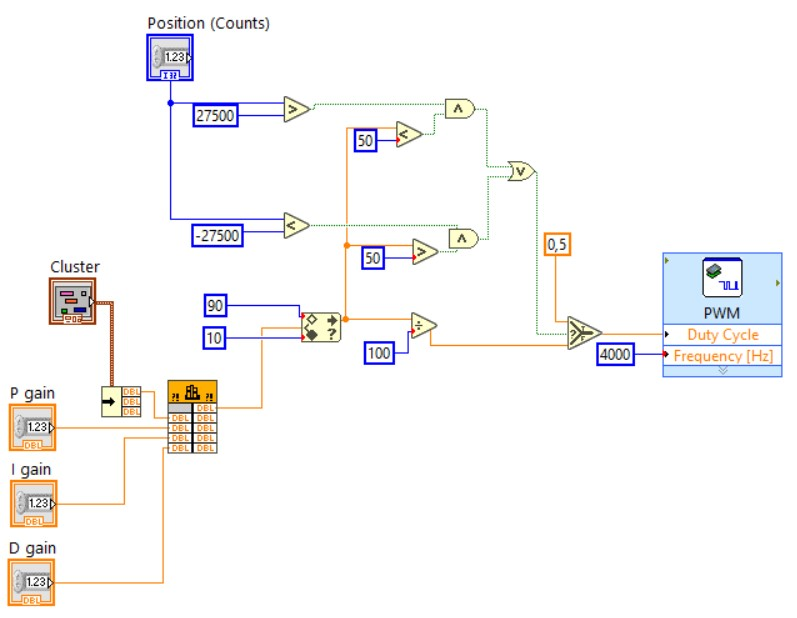
\includegraphics[width=6cm]{figure/labview_example.jpg}
    \caption{Example of a LabVIEW program.}
    \label{fig:lab-example}
\end{figure}

In addition to the LabVIEW code exemplified above, each program has a corresponding front panel where the user can interact with indicators and input controls. \cite{Andrade1998SoftwareTM}

\subsection{Integration With Text Based Languages} \label{theory:text_based}
Certain parts of a LabVIEW program may not be not suited for development in G, instead a text based language can be used and integrated into LabVIEW \cite{NationalInstruments2022BenefitsLabVIEW}. The integration can be either done by using the \textit{Formula Node} to write code with a syntax similar to C, or using the \textit{Call Library Function Node} to call a DLL (Dynamic-link library) or a shared library function \cite{Nationalinstruments2018CallNode}. The node takes in function parameters as specified in the node's settings, and uses their values when calling the specified function. When the called function completes, its value is returned and can be used by other parts of the LabVIEW program.

To be able to call a function using the Call Library Function Node the code must be compiled to either a DLL, or a shared library (a file with a .so filename extension) if using a Linux based target \cite{NationalInstruments2021CreatingTarget}. This library or DLL must then be uploaded to the target using for example SFTP (SSH file transfer protocol). If the target is Linux based the library should be uploaded to the \texttt{/usr/local/lib} directory. The name of the .so file should then be specified in LabVIEW inside the settings of the Call Library Function Node.

\section{MyRIO-1900}
The MyRIO-1900 is a device that combines multiple components such as an ARM processor, an FPGA (field programmable gate array)\footnote{An FPGA is an integrated circuit that consists of an array of logic gates, which can be configured by the user to create a specific hardware architecture \cite{Trochimiuk2021FPGAUsed}.}, as well as both analog and digital I/O (input / output) lines to help "students and educators complete real engineering projects in one semester" \cite{NationalInstruments2022MyRIO-1900}. The RIO architecture that the myRIO uses combines a processor with the I/O of the device via an FPGA \cite{NationalInstruments2020TheInnovation, NationalInstruments2022FromNI}. In the RIO architecture, the FPGA is connected directly to the I/O and is used to offload critical and intensive tasks from the processor \cite{NationalInstruments2022FromNI}. It also makes high throughput tasks that run on the FPGA more deterministic than if they had run on the processor.

\section{ESCON Motor Controller}
The ability to steer the front wheel of the bike is made possible by a the so called steering motor. The motor controller for the steering motor is an ESCON 50/5 designed by Maxon. This motor controller is a "PWM servo controller", which means it controls motors using Pulse Width Modulation (PWM). The PWM duty cycle range of the controller, meaning the range between which values the duty cycle can be varied, is 10\% to 90\% \cite{Maxon2021ESCONReference}.

\section{Steering Motor Encoder} \label{theory:encoder}
To measure the position of the steering motor, or how far the front wheel has been rotated, an encoder of the model HEDS-5540\#A11 is used. The encoder translates rotational motion into a digital signal by using a codewheel that interrupts a light beam when it spins \cite{AvagoTechnologies2014HEDM-55xx/560xHEDS-55xx/56xx}. The encoder outputs a waveform signal with a resolution of 500 counts per revolution.

\section{Inertial Measurement Unit (IMU)}
The bike features an Inertial Measurement Unit, or IMU, the specific model of IMU used is a Pmod NAV designed by Digilent. This device features an accelerometer and a gyroscope, as well as a magnetometer and a barometer, the latter pair of which are not used in this project. Both the accelerometer and gyroscope makes measurements in relation to the 3 Cartesian coordinate axes \cite{Digilent2017PmodManual}. The units of the given measurements are \textit{g} (circa $9.81 m/s^2$), and \textit{dps} (degrees per second) for the accelerometer and gyroscope respectively; these measurements are given separately for each of the three axes \cite{STMicroelectronics2015INEMOMagnetometer}.

\section{UART Communication}
Universal asynchronous receiver-transmitter, abbreviated to UART, is a device-to-device hardware communication protocol \cite{GraceLegaspi2020UART:Receiver/Transmitter}. UART is used to transmit and receive serial data between two devices, this is achieved with only two wires for the transmitting and receiving ends. Each of the UART devices has two signals named transmitter (Tx), and receiver (Rx); the transmitter of one device should be connected to the receiver of the other, and vice versa.

The UART interface is, as its name implies, asynchronous, meaning it does not use a clock signal for synchronization. Instead a bitstream is generated by the transmitter, which is sampled by the receiver; synchronization is accomplished by using the same baud rate on both of the devices.
The baud rate is the rate at which the information from the transmitter is sent.

Information is transferred in the form of a packet. The packet includes a start bit, the data frame, an eventual parity bit, and finally one or two stop bits. The start and stop bits indicate the borders of a packet, meaning its start and end. The data frame contains the actual data which is transferred, it has a maximum length of 9 bits if no parity bit is used, otherwise the maximum length is 8 bits. The parity bits can optionally be used to tell if the data frame has been changed during the transmission.

\section{VESC} \label{theory:vesc}
The VESC is a controller for brushless DC motors, also known as an ESC (electronic speed controller), created by Benjamin Vedder \cite{Vedder2014AESC}. Both the hardware and firmware are open source, and available on GitHub\footnote{The hardware and firmware can be found on GitHub at \url{https://github.com/vedderb/bldc-hardware} and \url{https://github.com/vedderb/bldc respectivly.}}. Communication with the ESC can be done using either a PPM signal, analog, UART, I2C, USB or CAN \cite{Vedder2016VESCESC}.

Vedder describes in \cite{Vedder2015CommunicatingUART} that when communicating with the controller using UART, each packet must be wrapped in bytes containing information about itself. The packet should begin with a start byte with a value of either 2 or 3, depending on the length of the packet. This should be followed by one or two bytes that specifies the length of the packet, followed by the payload. At the end, two CRC\footnote{CRC, or cyclic redundancy check, is used to detect if the payload contains errors \cite{Technopedia2020WhatCRC}.} checksum bytes, and a stop byte with a value of 3 should be added. Vedder continues to write that a UART packet has to be sent "at regular intervals" to prevent the ESC from timing out; this can be either a specific send alive packet, or any other command that sets a value. The content of \cite{Vedder2015CommunicatingUART} is based on an example for an STM32F4 discovery board which implements UART communication with the VESC in C \cite{Vedder2018Vedderb/bldc_uart_comm_stm32f4_discovery:UART}.

\subsection{VESC Tool}
The developer of the VESC has developed a graphical user interface for interacting with the motor controller \cite{Vedder2016VESCESC}. This tool should be used to configure the ESC to work with the specific motor that is being used. It can also be used to test the motor and display real time data like the current drawn, or the temperature of the VESC.

% METHODS
% CREATED BY MAGNUS GUSTAVER, 2020
\chapter{Methods}

The methods chapter describes the methods which have been used in an attempt to reach the end goal of the project. In addition to this, it is explained why these specific methods were chosen. Any additional information which might be needed to understand the used methods and reasoning behind them, is located within the previously presented theory section.

\section{Configuring the toolchain}

The tools and software used to program and control the Autobike had already been decided to a large extent by the previous groups which worked on the project, as well as other stakeholders. It was therefore necessary to install these tools before the previous work could be examined to the fullest extent, and before further work could commence.

The installation process of these tools, will be presented in the upcoming subsections. Installation steps of other pieces of software will also be presented, together with their purpose and the reasons behind why they were decided to be used.

\subsection{LabVIEW}

The parts of the Autobike software that were already written had been done in LabVIEW. The LabVIEW program itself was therefore installed with the purpose of being able to view this code. Since a MyRIO-1900 had been selected to run the code, a special toolchain of plugins and programs which supports the configuration the device, as well as uploading and running code on it, also had to be installed. These programs were all first party tools available on the National Instruments website\footnote{All the required software for developing for the MyRIO is available in the \textit{LabVIEW myRIO Software Bundle} available for download on the National Instruments website: \raggedright\url{https://www.ni.com/sv-se/support/downloads/software-products/download.labview-myrio-software-bundle.html}}, or in the package manager which was installed alongside LabVIEW. 

It should be noted that the installation of LabVIEW and the necessary packages is more time consuming and problem-ridden than what might first be expected. The installation itself is not uncommon to take multiple hours, especially if the computer's storage space runs out in the middle of an installation. This step was further delayed due to downloads from the National Instruments website not working for several days.

\subsection{Text editor and build tools for C code}

Some of the more advanced algorithms used in the Autobike were better suited to be written using C code, and called by the main LabVIEW program. These algorithms include code written for another version of the bike with the purpose of controlling the steering motor, as well as code needed in the communication with the forward motor.

To be able to use C code with LabVIEW, a toolchain capable of both writing C code, but also (cross) compiling it, was required. The toolchain would also need to create shared libraries as well as uploading these to the target. The selected software, and the rationale behind the choices are further discussed below.

\subsubsection{Text editor / IDE: Visual Studio Code}

National Instruments has published a guide for setting up a C development toolchain using the IDE (integrated development environment) Eclipse \cite{NationalInstruments2021GettingEdition}. However due to preferential reasons and the project members' familiarity with Visual Studio Code (VS Code), it was chosen as the editor instead of Eclipse. 

The basics of the previously mentioned guide can still be followed even though the details differ. There is a guide published on the National Instruments forum that describes how VS Code can be set up to work with the MyRIO as well \cite{J2020NICode}. Although this is not an official guide, it is authored by a NI employee. After installing VS Code, the \textit{C/C++ for Visual Studio Code} extension is recommended as it allows for code-completion aids and debugging capabilities for code written in C \cite{VanLiew2022C++Code}. 

\subsubsection{Compiler and Build Tools: GCC, CMake and Ninja}

Before the C code can be called from within LabVIEW when it is running on a MyRIO, it must first be compiled and built into a shared library as mentioned in section \ref{theory:text_based}. The previously mentioned guide for setting up VS Code to develop for a MyRIO also goes through how to set up the needed build tools \cite{J2020NICode}. 

The compiler used in the guide is a version of GCC made to run on Windows, and compile the code for Linux running on ARMv7; this compiler is used since VS Code is running on a computer using windows and the myRIO has an ARM processor. To aid the build process CMake, which is "a family of tools designed to build, test and package software", is used to generate makefiles \cite{Kitware2022CMake}. These files can then be used by Ninja, a build system, to run the compiler and create a shared library or \texttt{.so} file \cite{Hasse2022NinjaSpeed}.

\subsubsection{FTP Client: Filezilla}

When the shared library or \texttt{.so} file has been created, this file needs to be transferred to the myRIO. To accomplish this, the guide recommends Filezilla, which is a "cross-platform FTP, FTPS and SFTP client" \cite{FileZilla2022ClientFeatures}. Filezilla was used to connect to the myRIO and upload the files as described in \ref{theory:text_based}.

\section{Examining Previous Work and the Current State of the Project}

When the tools necessary for viewing and running LabVIEW code had been set up, the existing code was examined and tested. This was done in order to learn what parts of the Autobike's software had not yet been completed. It was concluded that all hardware except the forward motor could be interacted with in some way from the main LabVIEW program. 

All sensors, including the GPS, gyro, accelerometer, hall sensor (for measuring the forward speed), and position sensor (to measure the steering wheel position) was visually represented by graphs or similar on the LabVIEW front panel. The steering motor duty cycle could be controlled using a slider, and the emergency stop could stop the program except for in some edge cases (it should however be noted that the emergency stop always physically broke the circuit).

In addition to the main LabVIEW program, several other VIs were present in the folder handed over by the previous project group. Some of these were used as sub-VIs in the main program, but the majority of them seemed to be test code that had been used during the development process. One of these programs appeared to be an attempt at communicating with the forward motor; attempts to make the code to work were however unsuccessful, as further described in \ref{method:forward}.

\section{Steering Motor}

At the start of this project progress related to being able to control the steering motor had already been made by the previous project group. Excluding the hardware, LabVIEW code which could communicate with the steering motor controller, using a PWM signal, had already been completed. The duty cycle of the PWM signal had a value ranging from 0\% to 100\%, where a values above 50\% would rotate the motor clockwise, and values below 50\% rotate the motor anti-clockwise, a value of 50\% would stop the motor. 

The code consisted of three states: a start state, the control loop, and the end state. The start state made sure the motor was still and thereafter disabled the pin where the signal was sent, and waited until the user told the motor to start with a "Go" button. After being told to start, the control loop would be entered and the pin was enabled, which allowed the user to control the speed and direction of the motor using a slider; the slider changed the PWM signal sent to the motor controller. Finally the end state would be entered if a stop signal was given, for example by activating the physical emergency stop button, this state also stops the motor and disables the pin.

Testing the code by starting the program, pressing the "Go" button, and changing the PWM signal, the code proved to be working as intended; the motor could rotate in both directions and change speed accordingly. Therefore it was decided the code was going to be used, with minor alterations in the form of exchanging the slider for the previously mentioned control algorithm.

The following subsections describes the methodology and process of completing the software for the steering motor. This includes identifying and translating relevant code from another version of the Autobike, using the gyroscope built into the IMU together with the algorithm to control the steering motor, and implementing safety limits to the motor's range of motion.

\subsection{Transferring Control Algorithm From the Black Bike}

To reach the end goal of creating a bike which can balance on its own, code that was written for the other version of the bike, the so called black bike, were to be converted as to work with the current version which this project relates to. The software for the black bike had been written completely in Python, however it still used a MyRIO. 

Before the code could be used, the parts of the code which are relevant to the current bike, had to be identified. This process, followed by the conversion of the code to C, and its integration with LabVIEW is described below.

\subsubsection{Identifying Relevant Code}

Since the software used on the black bike was written entirely in Python, a large amount of the code had the same or similar functionality as the LabVIEW code for the red bike. For reference, the folder that was received contained in total 156 python files with a combined 20 253 lines of code\footnote{As reported by running the following commands in a Linux terminal:\\\texttt{find . -mindepth 1 -type f -name "*.py" -printf x | wc -c}\\\texttt{wc -l `find . -type f -name "*.py"`}}. Code which was used for loading simulations from CSV files were also present in most of files. From this it could be concluded that almost all of the received code was not relevant for the red bike and would not have to be used.

Trajectory tracing is also not a part of this project's goal, meaning the only part of the code that would be needed was the code which relates to keeping the bike stable. This code was located in the file \texttt{controller.py} and more specifically in the function \texttt{keep\_the\_bike\_stable}. The function also called another function, \texttt{update}, which implemented a PID controller in parallel form according to:

\begin{equation*}
    u(t) = K_p e(t) + K_i \int_{0}^{t} e(t)dt + K_d \frac{de}{dt}
\end{equation*}

The value returned from this function is then further sent to another function, named \texttt{controller\_set\_handlebar\_angular\_velocity}. This final function calculates the angular velocity of the motor based on some safety limits, and calls a function to convert the angular velocity to a duty cycle. In Python, this conversion is done using the \texttt{interp} function from the \textit{NumPy} library with the velocity on the x-axis, and PWM on the y-axis. In C this as been converted to \texttt{50 + rpm * 40.0 / 1000.0}, which gives a value between 0 and 100 when \texttt{rpm} is in the range of the motors angular velocity.

\subsubsection{Converting Python to C}

The previous project group that worked on the bike considered using a language called Cython to compile the Python code to C, and thus avoid having to manually convert the code \cite{AronssonKarlsson2022PROJECTAUTOBIKE}. The group mentions that the translation created code which was confusing and hard to understand, and is was concluded that "Cython is not useful for this project". It became further apparent that Cython was not needed after the relevant Python code had been identified. This conclusion was made based on the relatively small amount of code that would actually have to be converted. It was therefore decided that the code was going to be converted manually.

The conversion process started with a new C project being created and the identified Python functions being copied there. The code was then adapted to fit the C syntax, at the same time as irrelevant code was removed. This irrelevant code mainly included lines that was only called when a simulation file were present, but some code was also removed since it did not have any effect on the rest of the program (for example variables that were written to, but then never used). The safety limits were also removed and not implemented in the C code because it was decided they would be created in LabVIEW instead. This decision was based upon two reasons: to facilitate a better understanding and easier debugging of the code by having as much code written in LabVIEW as possible, as well as being able to use LabVIEW to log when a safety limit had been exceeded.

Another change that was made to the control algorithm when converting it into C code was the removal of code that depended on the time, i.e. the integral and derivative action in the PID controller. The integral of the error was instead implemented by adding the current error to the previous errors once every time the function was called. The derivative of the error was calculated as the difference between the current and previous error (the error the last time the function was called).

\subsection{Automating steering motor control}

To automate the control of the steering motor, meaning automatically calculating the duty cycle deciding which direction and how quickly the motor should rotate, a shared library file of the converted C code was created and uploaded to the MyRIO. The bike's roll rate\footnote{Roll rate in this case means the speed of which the bike rotates along its lengthwise axis.}, read from the IMU's gyroscope, as well as the three respective PID gains were then connected to a \textit{Call Library Function Node} in LabVIEW. The node was set to call one of the functions from the C algorithm. The called function uses these four parameters and returns the calculated duty cycle.

The received duty cycle can theoretically have a value outside the range of 10\% to 90\%. Because of this the duty cycle is coerced to fall within this range using the \textit{In Range and Coerce} function in LabVIEW.

For safety reasons the range which the wheel can turn within needs to be limited. By using the steering motor encoder, the position of the steering motor can be calculated in degrees from when the wheel is straight. As mentioned in \ref{theory:encoder} the encoder has a resolution of 500 counts per revolution, but when turning the wheel a full rotation, the resulting counts are approximately 220 000; the reason for this is unknown. Thus the resulting factor for converting between counts and degrees is $360 / 220000$. In LabVIEW the rotational position is then compared with a limitation, configured from the main program's front panel. The current limit is set to 45 degrees in each direction, as this is the limit used for the black bike. If the limit is exceeded the duty cycle is set to 50\%, meaning the motor should stop.
 
The duty cycle is then sent to a node in LabVIEW which creates a PWM signal. This signal replaces the previously existing slider and is in turn sent to the hardware pin (pin 19) which the steering motor controller is connected to.

\subsubsection{Calibrating Gyroscope}

When the automated control of the steering motor was tested, it was discovered that the motor rotated even if the bike was not moving. During an investigation of the graphs that plotted the gyroscopes values, it appeared as though the average value of the rotational rate around the roll axis was non-zero, even when the bike was stationary. This seems to be a case of a "constant bias error" \cite{Beavers2017TheGyro}.

To counteract the error, the bike was kept stationary over a time while the values returned from the gyroscope for the roll axis was recorded. The average of these recordings was then calculated and the negative of this average was added to the gyroscope's output to correct the error. It should be noted that the error or "constant bias error" might drift over time, meaning the error might change. If this occurs the average offset could be calculated again, or more sophisticated methods could be utilized as mentioned in \cite{Beavers2017TheGyro}.

\section{Forward Motor} \label{method:forward}

When the project was received, the main LabVIEW program contained no code with the purpose of controlling the forward motor. The reason for this code not being created was that "the command used for controlling the forward motor controller were not found" as described in the previous project's report \cite{AronssonKarlsson2022PROJECTAUTOBIKE}.

The MyRIO communicates using UART with the forward motor controller, which will be refereed to as \textit{the VESC} from this point on. The hardware necessary to control the forward motor using UART was implemented; the RX and TX wires had been connected between the MyRIO and the VESC, which in turn is connected to the forward motor. In LabVIEW there existed a VI which sent a command to the UART port connected to the VESC, however this program was undocumented and did not appear to work when it was tested.

Based on the previously created code, or lack there of, the LabVIEW code to communicate with the VESC using UART and consequently control the forward motor had to be created from scratch. This process with be described in the upcoming subsections. This process consist of configuring the VESC, encoding the correct UART command, successfully sending this command using LabVIEW, as well as some general testing and tuning.

\subsection{Configuring the VESC} \label{method:configuringVesc}

The development of the code meant to control the forward motor started with trying to use the already existing test program to send a UART command to the VESC. Even though the command appeared to match the description from \ref{theory:vesc}, the motor did not react. Why this was the case was unknown, which created doubts concerning which part of the setup caused the problem.

In an attempt to narrow down the cause of the problem, a computer running the VESC Tool was connected directly to the VESC via USB. Using this tool, an \textit{experiment} was made where a fixed RPM was sent to the controller. This resulted in a high pitched noise, as well as close to no movement of the motor.

It was hypothesized that the VESC was misconfigured in regard to the specifications of the forward motor. To try to fix this issue, the setup wizard built into the tool was used. In the wizard, the requested values and parameters was set to that of the motor \cite{Shimano2022DU-E6010}. The values which could not be found in the forward motor's data sheet were set to the recommended values. When running the same experiment as before and setting the motor's RPM to a fixed value, the motor now turned at what seemed to be the correct speed, without any screeching.

The VESC Tool is also used to make sure the VESC is set to use UART as its communication interface. This is done by changing the \textit{APP to Use} to UART under \textit{App Settings > General}. The baud rate can also now be accessed and changed, but is kept at the default value of 115 200 bps.

\subsection{Encoding UART command}

The UART communication with the VESC is based on sending various commands which should make the motor react in a certain way. Apart from the blog post by Vedder cited in section \ref{theory:vesc} as well as his example for the STM32F4 discovery board, there exists no documentation for how the UART commands sent to the VESC should look. 

The first attempt at encoding a UART command was made almost entirely in LabVIEW by setting a RPM value in the front panel, flipping its endianness, and wrapping it in start and stop bytes as well as checksum bytes. The payload was also split into separate bytes in the same way as in Vedder's example. Due to lacking documentation regarding the UART implementation, and there being no easy way of knowing exactly what bytes a correctly encoded message should contain, this method was later abandoned.

It was instead decided that a shared library would be created based on the example made by Vedder; the shared library could then be called using a \textit{Call Library Function Node} in LabVIEW. This method circumvented the problem of having to write the communication in a, for this purpose, undocumented language. Instead the correct command could be returned from a C function based on an inputted RPM value. 

To create this library which could be called by LabVIEW, the code that created the desired UART commands had to be identified. The functions to call and send specific commands was located in the \texttt{bldc\_interface.c} file. The three functions that have been adapted to work with the myRIO are \texttt{bldc\_interface\_set\_rpm}, \texttt{bldc\_interface\_set\_current}, as well as  \texttt{bldc\_interface\_send\_alive}. They have also been renamed to \texttt{setRpm}, \texttt{setCurrent}, and \texttt{sendAlive} respectively, to better represent  their new purpose. These functions was chosen since they were deemed to be the most useful commands related to controlling the forward motor. Functions later called by these functions have also been adapted and, in some cases, simplified. The functions \texttt{buffer\_append\_int32} and \texttt{buffer\_append\_float32} converts an integer or float values to a big-endian array, and \texttt{send\_packet\_no\_fwd} then calls a function to build and send the actual packet. In the adapted code, there is instead a function named \texttt{buildPacket} which builds and returns the packet. This function also calls \texttt{crc16} to calculate and add the checksum bytes. Finally the packet is copied to an array which is passed as a pointer to \texttt{setRPM} and \texttt{setCurrent}.

\subsection{Sending UART command using LabVIEW}

To create the UART command using LabVIEW, the desired RPM or current is sent to a \textit{Call Library Function Node} which is set to call the correct function from the C code, after it has been compiled and uploaded to the myRIO. The called function has an additional input parameter in the form of a pointer to an array. This array is initialized in LabVIEW, so that the pointer of it can be sent to the C code. When the C code runs, the pointer is used to populate the array with the values of the command which should be sent to the VESC. 

The actual transmission of the command is accomplished using the \textit{UART} block in LabVIEW. The block is configured to use the UART channel corresponding to the connection with the VESC, the baud rate is also set to 115 200 bps which is the same value as was previously configured in the VESC Tool. The transmission is placed inside of a loop to prevent the VESC from going to sleep.

The loop which which was desired to be used was a \textit{Timed Loop}, which executes at a precise rate specified by the user. Though due to problems with the program crashing, the type of loop was changed to a \textit{While Loop}; the cause of these crashes are unknown. A delay of one second was also introduced inside the loop to prevent it from throttling the rest of the system. The change of loop type did resolve the program crashing, though did also introduce another issue with recording loop times. This is further discussed in \ref{method:loopTimes}.

\section{Cleaning up and organizing the code}

In an attempt to make it easier for both the current and future people working on the Autobike project, all of the LabVIEW and C code that is used has been moved into a single folder. Previously it was separated into two different folders which had to be placed in specific locations on the development computer for LabVIEW to be able to detect them. The folder has also been uploaded to a monolithic public GitHub repository\footnote{https://github.com/Hannnes1/autobike}. The purpose of this is to make it easier to collaborate on the code, as well as making it possible to keep track of changes. It should also make it easier for others to take over development of the bike, as this was previously unnecessarily tedious. However, due to how LabVIEW functions, there is still one file which has to be manually located when opening LabVIEW on a new computer, this file is located inside \texttt{labview/bin} together with all other files that the LabVIEW project uses.

The LabVIEW code that was received from the previous project group has been cleaned up, meaning that the main program has been separated into several sub-VIs, and unused code has been removed. The main advantage of creating sub-VIs is to reduce the area which the LabVIEW code uses; a large area makes it hard to locate code since you can not zoom inside LabVIEW. The code that has been removed are mainly VIs that were either old versions of the main VI, or old code used for testing individual components (presumably from before this was integrated into the main VI). By removing unused VIs the potential confusion about what a VI does, and which VI is the most recent one, is mitigated.

Care has also been taken to document the new code that has been written, as well as the old code, so that anyone can continue the development process without having to interpret all of the code without any guidance. In addition to writing comments inline in the C and LabVIEW files, a \texttt{README.md} file has also been created in the root of the repository. This file lists all the folders that are currently present and explains their purpose. When relevant, this file also contains instructions for how the content of the folder should be used.

\section{Logging of Control and Sensor Signals} \label{method:logging}

With the purpose of being able to record and log the control and sensor signals of the bike, a logging system had to be created. This system would allow for future logs of a test being plotted and analyzed, helping the tuning process of the system. The logs could also be used to troubleshoot potential problems with the bike's performance.

In this specific case to be able to examine the data from performed tests, values from sensors, actuators, and the balancing algorithm added to the logging system. LabVIEW has built in functionality for this using the \textit{TDMS file format} \cite{NationalInstruments2022TheFormat}, which includes blocks for opening and creating, streaming to, and closing TDMS files. These files can then be opened using a number of different methods. Some of these methods include a special LabVIEW VI, Excel, or MATLAB using the \textit{Data Acquisition Toolbox}. 

In the main LabVIEW program used on the bike, a TDMS file is either created or replaced in the specified location using a \textit{TDMS Open} block. In each location where data should be logged, a \textit{TDMS Write} block is added and a group name and channel name is specified. Data is inputted as an array where each element corresponds to one channel (when the data layout has been specified as \textit{interleaved}). Each time that data is sent to the TDMS block, new data points are added to the channels. Therefore by placing the block inside of a loop, data from each iteration of the loop will be logged to the file. When a test is completed and all of the test data has been recorded, the file is closed using a \textit{TDMS Close} block before the program finishes.

MATLAB was chosen as the method for analyzing the data which the logging system gathers. MATLAB was specifically chosen due to the flexibility it grants regarding how the data can be presented. The code to do perform the plotting is presented in appendix \ref{code:plotting},

\section{Testing and Validating}

During the development of the bike's software, several tests have been done continuously to ensure that the developed features worked as expected. These tests include both simpler and informal tests designed to validate the bike's most basic functions, and more formal tests where values of different signals were logged. A test protocol was also constructed to be able to recreate the performed tests. It is the methodology behind these tests which will be presented in this section. The corresponding results are presented in the upcoming chapter \ref{results}.

\subsection{Testing the Basic Functionality of the Motors}

The first tests which were performed consisted of running the two motors at constant speeds. These tests where made to ensure that the motors worked as expected, without fluctuating speeds. 

For the steering motor the first test was performed by running the existing LabVIEW code and adjusting the duty cycle of the motor using the slider on the front panel. During this test the bike's front wheel was suspended midair so it could rotate freely. After the balancing algorithm had been created and connected to control the steering motor, it was tested by leaning the bike and examining if the steering motor rotated in the same direction. This purpose of the latter test was only to insure the steering motor reacted when the roll rate of the bike changed, and not that the calculated control signals were reasonable.

The first test of the forward motor was described in \ref{method:configuringVesc}. Summarized, it was performed by using the VESC Tool to run the motor at a fixed RPM. Later on, when the code to send UART commands via LabVIEW had been created, a fixed RPM was instead sent to the motor via one of these commands. Both of the tests mentioned above were performed when the bike was stationary and elevated into the air, this to insure the bike would not start moving.

\subsection{Testing the Balancing Algorithm}

After concluding that both motors worked separately, the balancing algorithm was able to be tested with both motors running. Two types of tests were performed, the first using a bike roller, and the second allowing the bike to move unaided. Both of these tests are described in the subsections below.

\subsubsection{Bike Roller Test}

The bike roller test made it possible to replicate the effects of going forwards while not requiring a large amount of space. The test consisted of placing the bike on the roller and turning on both motors. For safety the bike was held, though this was done whilst trying to not manually interfere in its movement. The aim of this test was to examine if the motors worked in tandem, and if it seemed as the bike could potentially balance on its own. It should be noted that a large restricting factor of this test is the limited space the bike can move sideways before reaching the boundary of the roller.

\subsubsection{Unaided Test}

To test the bike using an approach closer to a real world environment, a series of tests were performed outdoors in a flat and open area. This test made it possible to drive the bike forward, as well as allowing it to move sideways, mitigating the limit of the previous bike roller test. To prevent the bike from falling and potentially being damaged, two people ran alongside the bike ready to catch in the case it would fall.

For the purpose of being able to subsequently analyze the bike's behavior, the tests where both filmed and recorded using the logging system presented in \ref{method:logging}. Multiple tests were made with different values for the PID gains, to see how changing these values would affect the bikes performance. 

The data which was chosen to be recorded, logged and plotted with MATLAB include the position and speed of the steering motor, the duty cycle sent to the steering motor, as well as the roll rate of the bike. The results of some of these tests are shown in section \ref{results:balancing}.

\subsection{Testing the Program's Loop Times} \label{method:loopTimes}

While not being apart of the project's aim in itself, the performance of the program is of interest. This is because the bike's balancing could potentially be impacted if parts of the program takes too long to run. To be able to measure the performance, the time to run one iteration of each loop in the LabVIEW program was recorded. These times are then added together to get a total loop time for the program. The members of the previous project group have done a more in depth examination of this performance, which means that the values which are retrieved during the current testing can be compared with those values. It should be noted that because a while-loop had to be used for the forward motor control, the time it takes to run can not be measured. However, since a delay of one second runs in the loop, that is the loop time unless the other code in the loop takes longer to compute (which it does not). Additionally, the loop time of the forward motor control does not matter in this stage of the project, since the speed of the motor will be kept constant.

\subsection{Test Protocol}

To simplify the process of replicating the tests, a testing protocol was created. All of the tests which had been previously performed which also were seen as reasonable to replicate were added. Some suggestions for tests which could help calibrate the balancing algorithm for either the red bike or other future versions were also added. The testing protocol includes descriptions of the tests, the desired results and eventual comments. The protocol can be found in appendix \ref{testingProtocol}.

% RESULTS
% CREATED BY MAGNUS GUSTAVER, 2020
\chapter{Results}\label{results}

This chapter presents the results of the project. Primarily the result corresponding to the main aim of the project, meaning the bike's ability to balance, will be presented. The results correlating to the sub-goals: how the bike performs with regards to the steering motor, forward motor and balancing algorithm are also presented. Finally the reasons behind the results, and the effects of them are discussed. Further more detailed results from the individual tests are documented in appendix \ref{testingProtocol}.

\section{Steering Motor}

The steering motor, when viewed as a standalone component fully works as intended. That is, it is disabled until the \textit{GO} button is pressed in LabVIEW, and then it can be controlled by changing the duty cycle between 10\% and 90\%. It also stops when the duty cycle is set to 50\%, as expected. When the emergency stop is pressed either physically or in the software, the duty cycle is set to 50\%, and the pin is disabled. 

When connecting the control of the steering motor to the balancing algorithm and safety limit, the motor turns towards the same direction which the bike is leaning, and the duty cycle is set to 50\% when the safety limits is reached. However, the steering wheel has the possibility of overshooting the safety limit because of the inertia of the steering wheel and handlebar. Whether this happens also depends on how fast it was rotating before the limit was reached.

The controls for the motors, separated into two boxes are depicted in figure \ref{fig:motorControl} below. Inside of the left box, the steering motor controls are located. In these controls there exist inputs for changing each of the PID gains labeled P, I, and D. The box also has a field for changing the angle limit (in degrees from when the wheel is straight). Below the controls mentioned above are outputs from the steering motor encoder which shows its current position, velocity and acceleration. For the purpose of calibrating the encoder, there exists a button which resets the encoder position whenever it is pressed. At the bottom of the box, the duty cycle sent to the motor from the balancing algorithm is shown. At the bottom right of the image, under the boxes, is the \textit{GO} button which starts the two motors.

\begin{figure}[ht]
    \centering
    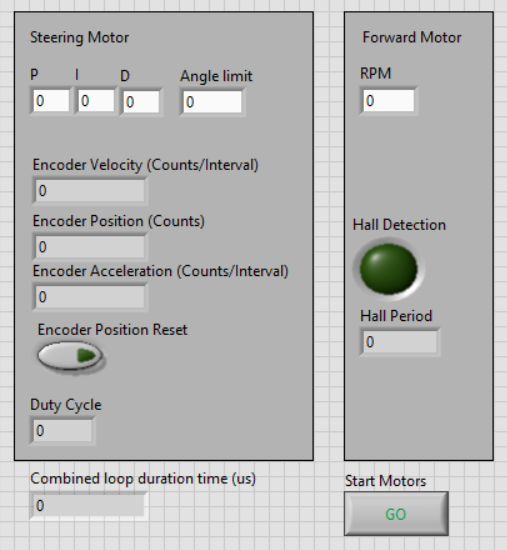
\includegraphics[width=7cm]{figure/motor_control.png}
    \caption{The motor controls in LabVIEW, with the steering motor control on the left side}
    \label{fig:motorControl}
\end{figure}

\section{Forward Motor}

The speed of the forward motor can successfully be set using the LabVIEW front panel as seen on the right side of figure \ref{fig:motorControl} above, and also changed while the program is running. The forward motor only starts when \textit{GO} is pressed, and it stops when the emergency stop is pressed; the same behavior that the steering motor has. 

The motor can not only be controlled by setting its speed directly, but also by changing its current. Controlling the motor using current can be accomplished if the function called by the \textit{Call Library Function Node} is changed to \texttt{setCurrent}. Additional methods of controlling the motor can be added by creating and calling additional C functions based on the example by Vedder.

\section{Balancing Algorithm} \label{results:balancing}

During the initial testing of the balancing algorithm, it was concluded that the steering motor behaved as expected in terms of rotation direction in relation to the roll rate of the bike. Meaning when the bike was leaned, the front wheel rotated towards the same direction. 

When the bike was then placed on the roller, it seemed as if the bike could stay upright for some time before it had to be caught to prevent it from falling. The algorithm would make the front wheel rotate to the correct direction, but the amplitude of these rotations was gradually increasing until the border of the roller was reached. A real, conclusive result could not be made from this test; the reasons for this are both because of human interference, as well as the narrow width of the roller.

The final and most reliable test of the balancing algorithm was done outdoors as described in \ref{method:unaidedTest}, and the P gain was set to 5 (I and D were set to 0). The data from these tests, recorded with the logging system, are presented in the images below.

\begin{figure}[H]
    \begin{subfigure}{.5\textwidth}
        \centering
        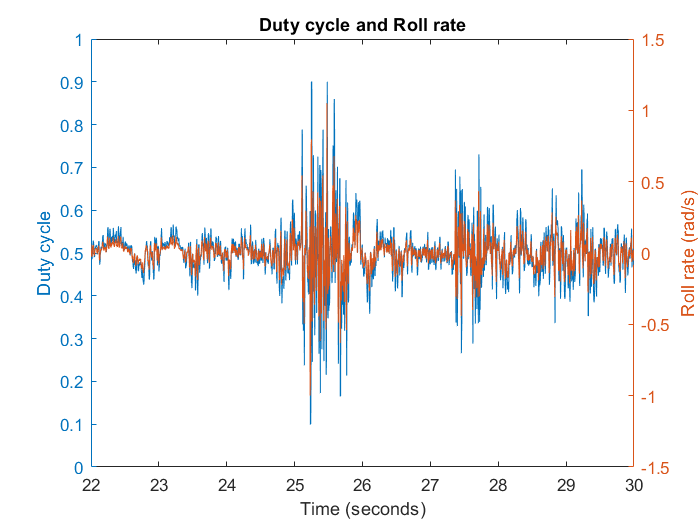
\includegraphics[width=\textwidth]{figure/dutyAndRoll.png}
        \caption{The roll rate of the bike and duty cycle sent from the balancing algorithm.}
        \label{fig:dutyAndRoll}
    \end{subfigure}
    \begin{subfigure}{.5\textwidth}
        \centering
        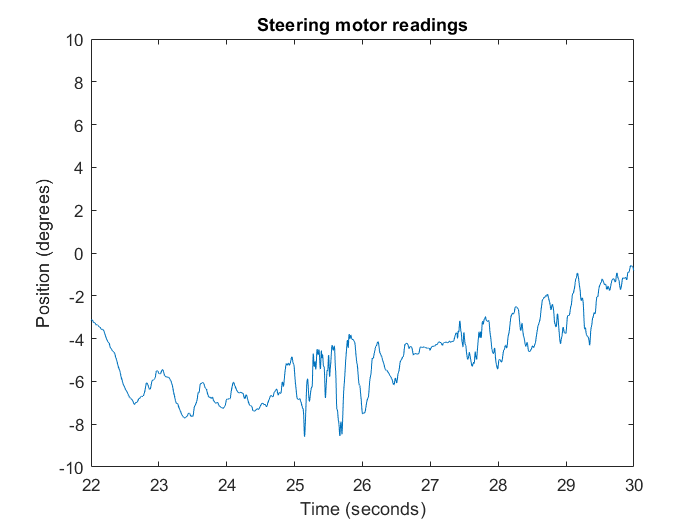
\includegraphics[width=\textwidth]{figure/motorPosition.png}
        \caption{The position of steering motor during the test.}
        \label{fig:motorPosition}
    \end{subfigure}
\caption{Plotted data from the final test.}
\label{fig:finalTest}
\end{figure}

In the test presented above the roll rate of the bike is relatively stable around 0. There only major deviance is around the 25:th second, which is caused by the bike passing over a bump in the road. As seen in blue line in figure \ref{fig:dutyAndRoll} which represents the duty cycle, the rapid change in duty cycle also leads to a change by the control algorithm as a correction. The steering motor has some oscillations with and amplitude of about $2\degree$ and period of roughly one second. That is however nothing which had any noticeable effect on the overall performance; the test lasted for 8 seconds, and had to be aborted when the bike drove too close to obstacles in the testing area.

\section{Loop Times}

For the loop time tests all of the bikes hardware was enabled so that all control signal calculations would be made, and the resulting time would be as accurate possible. The total loop time was recorded as being between \SI{2155}{\micro\second} and \SI{2420}{\micro\second}. Compared to the previous project group's measurements, the new loop times are at worst is \SI{240}{\micro\second} slower than the worst case before the logging system and C algorithms were added \cite{AronssonKarlsson2022PROJECTAUTOBIKE}.

\section{Discussion} \label{results:discussion}

The main part of the result which should be discussed is that the forward motor control stopped working before the final test. Meaning that the UART commands sent to the VESC did not result in the forward motor moving. The reasons for this are unknown, but the problem has been isolated to the VESC, perhaps a broken trace related to the UART connections are the cause. During the final test the bike was instead accelerated by pushing it, before being let go. Pushing the bike should though not affect the overall result, compared to if the forward motor was still working.

The improvement of the development experience is one aim which was presented in \ref{intro:aim}, this aim is however not mentioned above. The reason being this decision it that it is difficult to assess if the aim has been reached or not, since it can be considered individual to a certain degree. What can be said is that all of the code which is used has been moved to a single location, which should make it easier to find the code. It should also now be much clearer what code is the most recent one. The code itself has been organized and separated into sub-VIs which should also make it easier to find the relevant code, this in combination with more comments should also make it easier to understand it.

What the result of the final test, and the data in figure \ref{fig:finalTest} shows is that the bike can be kept stable by the balancing algorithm, even when the surface is uneven. There are some low frequency osculations of about the same frequency in all of the plotted data, which indicates that primarily the P gain of the PID controller could be tuned for better results.

There are some high frequency oscillations in the roll rate which might be caused by the IMU not being properly mounted, something which leads to vibrations; especially when the surface is uneven. Improper mounting of hardware can also be found elsewhere in the bike, which could be contributing to a worse balancing performance. These oscillations also creates high frequency changes in the duty cycle. Though this is generally not a problem since the steering wheel cannot change direction with such a high frequency; the dynamics of the bike could be described as acting as a low pass filter.


% CONCLUSION
% CREATED BY MAGNUS GUSTAVER, 2020
\chapter{Conclusion}

The main goal of the project was to develop the software for the Autobike so that it could balance on its own whilst driving forward. In practice this meant completing two sub-goals: implementing an algorithm which, using the roll rate of the bike, could calculate the correct duty cycle for the steering motor, as well as writing software to encode a UART command which then could be used to control the forward motor.

As described in the results, the two sub-goals as well as the primary aim of the project were reached. The forward motor can be controlled from LabVIEW, and the steering motor is controlled by the balancing algorithm. The balancing algorithm can also successfully keep the bike stable, at least until the forward velocity becomes too low. What this minimum velocity is has not been determined, and will vary depending on what the gains of the PID controller are. Even if the some pieces of hardware were not properly mounted, this did not affect the performance in any meaningful way in this stage of the development. If the controller were to be tuned further, the hardware should probably be securely mounted so that the best possible foundation is achieved.

The secondary goal of the project, improving the future development experience, is as previously discussed difficult to judge if it has been reached. The wording "improving" does not contain the degree of which this should be done, meaning any small improvement could be interpreted as reaching the goal. However, continuously during the project's development, files have been organized and cleaned up; both for the benefit of the current developers, but more importantly for any future developers. The question of whether this goal has been reached or not is therefore best judged by these future developers.

\section{Future work}

The priority for any future work should be to fix forward motor. Even if this is not something which affected the results of this report, the speed might become more important in the future if the current algorithms are improved, and additional ones are added. To accurately set the forward speed and to increase how far the bike can be driven, the forward motor would have to work.

Future work should also be focused on improving the hardware, and primarily its mounting. The IMU is the most important hardware component for the balancing algorithm, and will therefore have to be mounted so that its axis aligns with the axis of the bike. It also has to be mounted in such a way that it does not move around or vibrate excessively.

% REFERENCES / BIBLIOGRAPHY
\emergencystretch=1em
\printbibliography

% APPENDICES
\cleardoublepage
\appendix
\setcounter{page}{1}
\pagenumbering{Roman}			% Capitalized roman numbering starting from I (one)

\chapter{LabVIEW User Manual} \label{labviewManaul}

This appendix goes through the main LabVIEW program, and explains how it should be used from a user's perspective. The program is launched by opening project found under \texttt{labview/red\_bike.lvproj} in LabVIEW 2019. Later versions might work as well, but the 2019 version is recommended for the best compatibility. Inside the project, open \texttt{myRIO-1900/bin/TestMain.vi}. The first time the program is opened on a new computer, LabVIEW might give a warning that a \texttt{.lvbitx} file could not be found. This file is located in \texttt{labviw/bin}, and can manually be pointed to when requested.

With the program opened, the controls which can be interacted with to control be bike are located in the top left of the front panel. These controls are shown in image \ref{fig:labviewControls} below.

\begin{figure}[H]
    \centering
    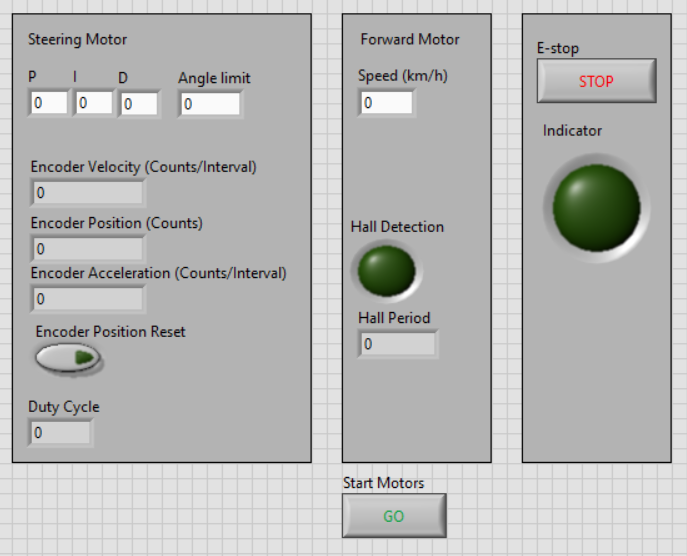
\includegraphics[width=10cm]{figure/labview_controls.png}
    \caption{The controls which can be interacted with in the LabVIEW front panel.}
    \label{fig:labviewControls}
\end{figure}

In the leftmost box in the picture contains the controls for the steering motor. Here, the PID gains and the angle limit (in degrees from the center), can be changed. Below this are the readouts from the encoder, and a button to reset its position. This button should be pressed when the front wheel is straight to calibrate the encoder before starting any of the motors. At the bottom of the box is the duty cycle which is sent from the balancing algorithm to the steering motor.

The middle box at the center of the image contains the controls for the forward motor. The only thing which can be changed here is the RPM, note that the RPM are measured in relation with the pedals (for the red bike). Below the forward motor controls is a button which starts the two motors. It should be mentioned that the program can still be running without affecting the motors, if this button is not pressed.

At the right is a software implementation of the emergency stop. From the program's perspective, this acts exactly as if the hardware emergency stop was to be pressed.

The path to the log file (including its desired name) can be specified in the text field which is located at the absolute bottom of the image. The path leads to a file \textbf{on the MyRIO} where the LabVIEW program is running, and must be inside the \texttt{/home/lvuser/} directory. This is due to the program not having \textit{sudo} privileges in the Linux OS which is running on the device. If no file exists in the specified path, a file will be created. If a file does exist, it will be replaced and overwritten when the program starts. It is therefore recommended to change the file name before each time the program is to be run. To open the log files, they have to be downloaded from the MyRIO using for example FileZilla, and then opened using any of the methods mentioned in \ref{method:logging}.

The rest of the front panel consists of the values from the various sensors. On the right of the controls depicted in the figure above are three graphs illustrating the values from the IMU's gyroscope. The topmost graph corresponds with the roll rate which is used by the balancing algorithm. The front panel also shows GPS data and accelerometer values, these are however not used by any part of the program at the moment.

In summary, the following steps must be performed to start the bike and log its sensor and control signal data:
\begin{enumerate}
    \item Set the PID gains, and angle limit and RPM to something non-zero
    %\item Set the angle limit to something non-zero
    %\item Set the RPM
    \item Set the path to the logging file to somewhere inside the \texttt{/home/lvuser/} directory. For example \texttt{/home/lvuser/log1.tdms}
    \item Start the LabVIEW program
    \item Reset the encoder position when steering wheel is straight
    \item Press \textit{GO}
\end{enumerate}

Note that, to be able to start the LabVIEW program, the hardware emergency stop has to be up, and the hardware reset button has to be pressed. The program is ready when the light next to the reset button shines green.

\chapter{Code} \label{code}

This Appendix contains some of the code that have been used on the bike, or during the project. Some of the code, like the main LabVIEW program, is difficult to include in the appendix, but can be found on the Github repository together with all of the other code at the following URL: \url{https://github.com/Hannnes1/autobike}

\section{Balancing Algorithm} \label{code:balancing}

\lstset{
    language=C,
    basicstyle=\ttfamily\footnotesize,
    breaklines=true,
    morekeywords={matlab2tikz},
    keywordstyle=\color{blue},
    morekeywords=[2]{1}, keywordstyle=[2]{\color{black}},
    identifierstyle=\color{black},
    stringstyle=\color{mylilas},
    commentstyle=\color{mygreen},
    showstringspaces=false,%without this there will be a symbol in the places where there is a space
    numbers=left,%
    numberstyle={\tiny \color{black}},% size of the numbers
    numbersep=9pt, % this defines how far the numbers are from the text
    belowskip=3em,
}

\begin{lstlisting}
// balancing.h

#ifndef _BALANCING_H_
#define _BALANCING_H_

#define gearRatio 111.0
#define pi 3.141592

#define windupGuard 6

double integral = 0;
double derivative = 0;

double previousError = 0;

extern double stabilizeBike(double rollRate, double Kp, double Ki, double Kd);

double calculateSteeringPWM(double angularVelocity);

double pid(double reference, double currentValue, double Kp, double Ki, double Kd);

#endif
\end{lstlisting}

\newpage

\begin{lstlisting}
// balancing.c

#include "balancing.h"

extern double stabilizeBike(double rollRate, double Kp, double Ki, double Kd) {
    double steeringRate = pid(0, rollRate, Kp, Ki, Kd);

    // Send Steering Rate Reference value to steering motor controller
    double steeringPWM = calculateSteeringPWM(steeringRate);

    // Right now, the PWM is between 10 and 90 (this should be scaled down by a factor of 100)
    // if the angular velocity is between -0.9435 and 0.9435.
    // That means that the error can be at most +- 0.04715 if integral is 0.
    // (With Kp = 10, Ki = 10, Kd = 0)
    // Changing to Kp = 0.2, Ki = 0, Kd = 0, the error can at most be +- 4.715.
    return steeringPWM;
}

// Is there any reason not to calculate the PWM directly in the pid function?
// How can we even be sure that the angularVelocity matches reality?
double calculateSteeringPWM(double angularVelocity) {
    double rpm = -angularVelocity * 30 / pi * gearRatio;  // To comply with Right Hand Rule
    return 50 + rpm * 40.0 / 1000.0;
}

double pid(double reference, double currentValue, double Kp, double Ki, double Kd) {
    double error = reference - currentValue;

    integral += error;
    derivative = error - previousError;

    if (integral < -windupGuard) {
       integral = -windupGuard;
    } else if (integral > windupGuard) {
        integral = windupGuard;
    }

    previousError = error;

    return Kp * error + Ki * integral + Kd * derivative;
}
\end{lstlisting}

\newpage

\section{VESC UART Encoder}

\begin{lstlisting}
// common.h

#ifndef _COMMON_H_
#define _COMMON_H_

typedef unsigned char uint8_t;
typedef unsigned   uint32_t;
typedef short  int16_t;
typedef unsigned short  uint16_t;

unsigned short crc16(unsigned char *buf, unsigned int len);

#endif
\end{lstlisting}

\begin{lstlisting}
// common.c

#include "common.h"

// CRC Table.
const unsigned short crc16_tab[] = {
    0x0000, 0x1021, 0x2042, 0x3063, 0x4084, 0x50a5, 0x60c6, 0x70e7,
    0x8108, 0x9129, 0xa14a, 0xb16b, 0xc18c, 0xd1ad, 0xe1ce, 0xf1ef,
    0x1231, 0x0210, 0x3273, 0x2252, 0x52b5, 0x4294, 0x72f7, 0x62d6,
    0x9339, 0x8318, 0xb37b, 0xa35a, 0xd3bd, 0xc39c, 0xf3ff, 0xe3de,
    0x2462, 0x3443, 0x0420, 0x1401, 0x64e6, 0x74c7, 0x44a4, 0x5485,
    0xa56a, 0xb54b, 0x8528, 0x9509, 0xe5ee, 0xf5cf, 0xc5ac, 0xd58d,
    0x3653, 0x2672, 0x1611, 0x0630, 0x76d7, 0x66f6, 0x5695, 0x46b4,
    0xb75b, 0xa77a, 0x9719, 0x8738, 0xf7df, 0xe7fe, 0xd79d, 0xc7bc,
    0x48c4, 0x58e5, 0x6886, 0x78a7, 0x0840, 0x1861, 0x2802, 0x3823,
    0xc9cc, 0xd9ed, 0xe98e, 0xf9af, 0x8948, 0x9969, 0xa90a, 0xb92b,
    0x5af5, 0x4ad4, 0x7ab7, 0x6a96, 0x1a71, 0x0a50, 0x3a33, 0x2a12,
    0xdbfd, 0xcbdc, 0xfbbf, 0xeb9e, 0x9b79, 0x8b58, 0xbb3b, 0xab1a, 
    0x6ca6, 0x7c87, 0x4ce4, 0x5cc5, 0x2c22, 0x3c03, 0x0c60, 0x1c41,
    0xedae, 0xfd8f, 0xcdec, 0xddcd, 0xad2a, 0xbd0b, 0x8d68, 0x9d49,
    0x7e97, 0x6eb6, 0x5ed5, 0x4ef4, 0x3e13, 0x2e32, 0x1e51, 0x0e70,
    0xff9f, 0xefbe, 0xdfdd, 0xcffc, 0xbf1b, 0xaf3a, 0x9f59, 0x8f78,
    0x9188, 0x81a9, 0xb1ca, 0xa1eb, 0xd10c, 0xc12d, 0xf14e, 0xe16f,
    0x1080, 0x00a1, 0x30c2, 0x20e3, 0x5004, 0x4025, 0x7046, 0x6067,
    0x83b9, 0x9398, 0xa3fb, 0xb3da, 0xc33d, 0xd31c, 0xe37f, 0xf35e,
    0x02b1, 0x1290, 0x22f3, 0x32d2, 0x4235, 0x5214, 0x6277, 0x7256,
    0xb5ea, 0xa5cb, 0x95a8, 0x8589, 0xf56e, 0xe54f, 0xd52c, 0xc50d,
    0x34e2, 0x24c3, 0x14a0, 0x0481, 0x7466, 0x6447, 0x5424, 0x4405,
    0xa7db, 0xb7fa, 0x8799, 0x97b8, 0xe75f, 0xf77e, 0xc71d, 0xd73c,
    0x26d3, 0x36f2, 0x0691, 0x16b0, 0x6657, 0x7676, 0x4615, 0x5634,
    0xd94c, 0xc96d, 0xf90e, 0xe92f, 0x99c8, 0x89e9, 0xb98a, 0xa9ab,
    0x5844, 0x4865, 0x7806, 0x6827, 0x18c0, 0x08e1, 0x3882, 0x28a3,
    0xcb7d, 0xdb5c, 0xeb3f, 0xfb1e, 0x8bf9, 0x9bd8, 0xabbb, 0xbb9a,
    0x4a75, 0x5a54, 0x6a37, 0x7a16, 0x0af1, 0x1ad0, 0x2ab3, 0x3a92,
    0xfd2e, 0xed0f, 0xdd6c, 0xcd4d, 0xbdaa, 0xad8b, 0x9de8, 0x8dc9,
    0x7c26, 0x6c07, 0x5c64, 0x4c45, 0x3ca2, 0x2c83, 0x1ce0, 0x0cc1,
    0xef1f, 0xff3e, 0xcf5d, 0xdf7c, 0xaf9b, 0xbfba, 0x8fd9, 0x9ff8,
    0x6e17, 0x7e36, 0x4e55, 0x5e74, 0x2e93, 0x3eb2, 0x0ed1, 0x1ef0
};

// Calculates checksum bytes, based on payload and crc16_tab above.
unsigned short crc16(unsigned char *buf, unsigned int len) {
    unsigned int i;
    unsigned short cksum = 0;
    for (i = 0; i < len; i++) {
        cksum = crc16_tab[(((cksum >> 8) ^ *buf++) & 0xFF)] ^ (cksum << 8);
    }
    return cksum;
}
\end{lstlisting}

\begin{lstlisting}
// vescEncoder.h

#ifndef _VESC_H_
#define _VESC_H_

#include "common.h"

unsigned short crc16(unsigned char *buf, unsigned int len);

extern void sendAlive(uint8_t *array);

extern int setRpm(uint8_t* array, int rpm);

extern int setCurrent(uint8_t *array, int current);

void bufferAppendFloat32(uint8_t* buffer, float number, float scale, int *index);

void bufferAppendInt32(uint8_t* buffer, int number, int *index);

uint8_t *buildPacket(uint8_t *data, unsigned int len);

uint8_t txBuffer[512 + 6];

#endif
\end{lstlisting}

\begin{lstlisting}[escapeinside=``]
// vescEncoder.c

#include "vescEncoder.h"
#include "common.h"

#include <string.h>

static unsigned char buffer[1024];
`\newpage`
// Calculates command used to keep the motor alive.
extern void sendAlive(uint8_t *array) {
    int index = 0;

    buffer[index++] = 30; // Number correspondning to the keepAlive command.

    // Build the packet for the command.
    uint8_t *packet = buildPacket(buffer, index);

    // Copy calculated packet to the referance array.
	for (uint8_t i = 0; i < 10; i++) {
        array[i] = packet[i];
    }
}

// Calculates command used to set the current of the motor.
// Based on the given parameter "current".
extern int setCurrent(uint8_t *array, int current) {
	int index = 0;

	buffer[index++] = 6; // Number correspondning to the setCurrent command.

    // Rescale the current and swap its endianness.
	bufferAppendFloat32(buffer, (float) current, 1000.0, &index);

    // Build the packet for the command.
    uint8_t *packet = buildPacket(buffer, index);

    // Copy the calculated packet unto the referance array.
	for (uint8_t i = 0; i < 10; i++) {
        array[i] = packet[i];
    }
	return current;
}

// Calculates command used to set the rpm of the motor.
// Based on the given parameter "rpm".
extern int setRpm(uint8_t *array, int rpm) {
    int index = 0;

    rpm *= 250; // Convert to the actual RPM of the bike's pedals.

    buffer[index++] = 8; // Number correspondning to the setRpm command.

    // Swpan the endianness of the rpm.
    bufferAppendInt32(buffer, rpm, &index);
 
    // Build the packet for the command.
    uint8_t *packet = buildPacket(buffer, index);

    // Copy the calculated packet unto the referance array.
    for (uint8_t i = 0; i < 10; i++) {
        array[i] = packet[i];
    }
    return rpm;
}

// Builds the packet based on the given command and payload.
// See http://vedder.se/2015/10/communicating-with-the-vesc-using-uart/ for more information.
uint8_t *buildPacket(uint8_t *data, unsigned int len) {
    int bufferIndex = 0;

    if (len <= 256) {
        txBuffer[bufferIndex++] = 2;
        txBuffer[bufferIndex++] = len;
    } else {
        txBuffer[bufferIndex++] = 3;
        txBuffer[bufferIndex++] = len >> 8;
        txBuffer[bufferIndex++] = len & 0xFF;
    }

    memcpy(txBuffer + bufferIndex, data, len);
    bufferIndex += len;

    unsigned short crc = crc16(data, len);
    txBuffer[bufferIndex++] = (uint8_t)(crc >> 8);
    txBuffer[bufferIndex++] = (uint8_t)(crc & 0xFF);
    txBuffer[bufferIndex++] = 3;

    return txBuffer;
}

// Rescales the given "number" with "scale", before swapping its endianness with "bufferAppendInt32".
void bufferAppendFloat32(uint8_t* buffer, float number, float scale, int *index) {
    bufferAppendInt32(buffer, (int)(number * scale), index);
}

// Swaps the endianness of the given "number".
void bufferAppendInt32(uint8_t *buffer, int number, int *index) {
    buffer[(*index)++] = number >> 24;
    buffer[(*index)++] = number >> 16;
    buffer[(*index)++] = number >> 8;
    buffer[(*index)++] = number;
}
\end{lstlisting}

\newpage

\section{MATLAB Test Data Plotting} \label{code:plotting}

\lstset{
    language=Matlab,
}

\begin{lstlisting}
% Read all of the data in the TDMS file.
data = tdmsread("Logs/Test4.tdms");

%% Encoder

% `data` contains one cell per group. Each cell contains
% a table with one column per channel. In this case, the
% first channel in the first group contains the time, 
% and the second channel contains the position etc.
time1 = table2array(data{1,1}(:,1));
position = table2array(data{1,1}(:,2));
velocity = table2array(data{1,1}(:,3));

figure;
yyaxis left;
% 611 is the conversion ratio from counts on the encoder
% to degrees.
plot(time1-time1(1),position/611);
ylim([-20,20]);
ylabel("Position (degrees)");
hold on;
yyaxis right;
plot(time1-time1(1),velocity/611*1000);
ylim([-50,50]);
ylabel("Velocity (degrees/s)");
xlabel("Time (seconds)");
xlim([7,11.5]);
title("Steering motor readings");
hold off;

%% Gyro
time2 = table2array(data{1,2}(:,1));
rollRate = table2array(data{1,2}(:,2));

figure;
plot(time2-time2(1),rollRate);
ylabel("Roll rate");
xlabel("Time (seconds)");
title("Gyro");

%% Steering motor

time3 = table2array(data{1,3}(:,1));
pwm = table2array(data{1,3}(:,2));

figure;
plot(time3-time3(1),pwm);
ylim([0,1]);
ylabel("Duty cycle");
xlabel("Time (seconds)");
title("Steering motor control");

%% Combined

figure;
yyaxis left;
plot(time3-time2(1),pwm);
ylim([0,1]);
ylabel("Duty cycle");
hold on;
yyaxis right;
plot(time2-time2(1),rollRate);
ylabel("Roll rate");
ylim([-10,10]);
xlim([7,11.5]);
xlabel("Time (seconds)");
title("Duty cycle and Roll rate");
\end{lstlisting}

% CREATED BY MAGNUS GUSTAVER, 2020
\chapter{Testing protocol} \label{testingProtocol}

The table below depicts the testing protocol table. For each test there is a corresponding description, an expected result, potentially a comment, as well as a validated column.

\begin{table}[h]
    \centering
    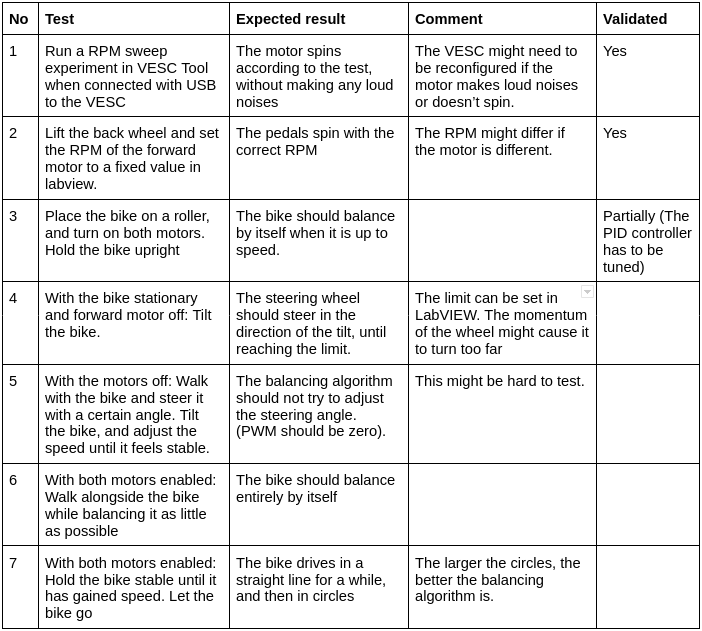
\includegraphics[width=\textwidth]{figure/testing protocol.png}
    \caption{The testing protocol. The \textit{Validated} column has been filled in for the tests which have been completed so far.}
\end{table}

% CREATED BY MAGNUS GUSTAVER, 2020
\newpage

%Header Last Page
\vtop{
    \null\vspace{-47.5mm}
    \centerline{\textcolor{thesisHeaderColor}{\rule{1.28\textwidth}{28mm}}}
    \null\vspace{-9mm}
    \centerline{\textcolor{headerBrown}{\rule{1.28\textwidth}{4pt}}}
    \vspace{187mm}
    \if\ThesisType M
    \centerline{
\includegraphics[width=0.2\pdfpagewidth]{figure/auxiliary/AvancezChalmersU_black_centered.eps}}
    \fi
    \if\ThesisType B
    \centerline{
\includegraphics[width=0.2\pdfpagewidth]{figure/auxiliary/AvancezChalmers_black_centered.eps}}
    \fi
    \vspace{-220mm}
}

\addtolength{\voffset}{2cm}
\renewcommand{\familydefault}{\sfdefault} \normalfont % Set cover page font
\pagestyle{empty}
\vspace*{-4.8cm}
\noindent
\textcolor{white}{\footnotesize \textbf{DEPARTMENT OF ELECTRICAL ENGINEERING}\\
\textbf{CHALMERS UNIVERSITY OF TECHNOLOGY} \\
Gothenburg, Sweden \\
\href{www.chalmers.se}{\textcolor{white}{www.chalmers.se}}}



\end{document}